\documentclass[12pt,twoside]{report}
\usepackage[utf8]{inputenc}
\usepackage[round]{natbib}
\usepackage{graphicx}
\usepackage{amsmath}
\graphicspath{{images/}}
\usepackage{caption}
\usepackage{subcaption}
\usepackage[left=27mm,right=27mm top=27mm, bottom=27mm]{geometry}
\usepackage[ruled,vlined]{algorithm2e}
\usepackage{fancyhdr}
\pagestyle{fancy}
\fancyhead{}
\fancyhead[LO,LE]{\leftmark}
\fancyfoot{}
\fancyfoot[CO,CE]{\thepage}
\renewcommand{\headrulewidth}{0.2pt}
\renewcommand{\footrulewidth}{0.2pt}

% Redefine plain page style (used for chapter first pages)
\fancypagestyle{plain}{
    \fancyhf{} 
    \fancyfoot[CO,CE]{\thepage}% Footer content for chapter pages
    \renewcommand{\headrulewidth}{0pt} % Remove header rule
    \renewcommand{\footrulewidth}{0.4pt} % Footer rule (adjust thickness if needed)
}


\usepackage[style=authoryear]{biblatex}
\addbibresource{references.bib}



\title{Tractable inference for latent ability in competitive games:approximating Bayesian rank-ordered models using a simpler proportion model.}\\

\author{Marta Sech}
\date{December 22nd 2023}

\begin{document} 
$-- Provides configuration of document metadata for writing the title block. 
$-- Note that in addition to these templates and partials, Quarto will also make normalized authors and affiliations data available to the template, 
$-- making is easy to write custom title blocks against a standard schema.
$--
$-- %%%% TODO %%%%%
$-- Customize is needed, otherwise remove this partials to use Quarto default one
$-- %%%%%%%%%%%%%%%%

$-- PLOS does not add title outside of document body. We make this template empty 


\tableofcontents

\chapter{Introduction}
In many contexts we come across data that take the form of rankings. This type of data is present, for example, in researches concerning the preferences of individuals for different candidates in elections ( \cite{stern1993probability} \cite{koop1994rank} or for different consumer goods (\cite{beggs1981assessing}). In these cases, the aim is usually to investigate individual's choice decisions  (\cite{yu2019analysis}).  Another area where ranking data are common is in sport  and game analytics, where the goal is rather to use game results to estimate the ability of competitors. This is done for example in \cite{van2023bayesian} with Formula One race results, in \cite{ali1998probability} with horses-races or in \cite{graves2003hierarchical} with NASCAR competitions. \\
\\
If ranking data want to be analysed, models tailored for this typology of data are needed. There are several known parametric models in the literature. One of the most popular is the one proposed by \cite{luce1959possible} and \cite{plackett1975analysis}. Rank- Ordered Logit models (ROL) (\cite{hausman1987specifying}) extended it by incorporating covariates. \\
\\
Although the validity of the ROL models has been widely acknowledged, their execution can be complex in the practice for two reasons. The first one concerns the estimation, which can become computationally burdensome when the number of competitors to be ranked is large: \cite{alvo2014statistical}  report fifteen competitors as the threshold in this sense. Secondly, the interpretation of parameters is not straightforward, as it requires multiple steps to have them related back to the outcome (refer to  Algorithm \ref{alg:sim} to understand how the rank of a competitor can be recovered from his ability parameter).\\
\\
These challenges lead researchers to use alternative models for rating competitors. For example, a linear regression was used in \cite{eichenberger2009best}, a multilevel approach in \cite{bell2016formula} and a Beta regression in \cite{stern2008ranking} \\
The approach that will be investigated in this paper is based on the transformation of the rank order of competitors given in each game into a proportion of competitors beaten for each player. This outcome can then be modeled using a Beta regression with dummies variables representing competitors as predictors. The associated regression coefficients can then be used to provide the desired rating of competitors. The downside of this approach is that it makes the incorrect assumption that the achieved ranking is (conditionally) independent of the achieved rank of the other competitors in the game. For example, if an averaged-skilled runner enters a local competition, he may ends up in the best positions and achieve a high proportion of competitors beaten. Nonetheless, if the same athlete enters a national level race where only the best contenders compete, his performance will be worse and so its proportion of competitors beaten.\\
\\
In summary, the Rank-Ordered Logit model and  Beta regression both have advantages and disadvantages in their use. Which one is preferable and when is currently unknown. In this project we will try to evaluate this and therefore answer the following research question: under which conditions (if any) is a proportion model a reasonable approximation for a complex rank-ordered model? \\
\\
This report is structured as follows: first, in Chapter 2  additional background about models for ranking data is provided and Plackett-Luce model is introduced and explained. In the same chapter we also discuss the use of alternative  models, with a particular focus on Beta regression. In Chapter 3, the simulation study  used to answer the research question is delineated, alongside with the  methodology used to compare the two models. In Chapter 4, we present simulations results and insights while in Chapter 5 we apply both models to a real-world example for illustration purposes. We end the paper with conclusions and suggestions for researchers who want to perform inference on ranking data.


\chapter{Theoretical background}
\section{Models for ranking data}
Literature offers a wide range of parametric models to deal with ranking data, nicely summarised by \cite{critchlow1991probability}. These models are typically explained in terms of judges' preferences for different items. As the framework context of this article is competitive games, in this project games assume the role of judges and the competitors participating in each game represent the ranked items.\\
\\
If competitors' abilities want to be inferred from ranking data,\cite{bradley1952rank} model can possibly be used. This model is suited to analyse paired-comparison data, for which the probability that a player $i$ wins against another player $j$ $p_{ij}$  is modeled as: 
\begin{equation*}
p_{ij} = F(\lambda_{i}-\lambda_{j}),
\end{equation*}
where $F$ is the logistic function and $\lambda_{i}=log⁡(\alpha_{i})$ for all $i$. $\alpha_{i}$ is a positive value representing the ability of the $i-th$ competitor and can therefore be used to rate competitors in head-to-head competitions. Nonetheless, this model can also be applied to a multi-competitor game context where $n$ competitors compete against each other in each game. This is done by converting the ranking of competitors in each game into the $n(n-1)/2$ set of possible paired comparisons between them. Still, this may not represent the most optimal approach, as it would cause a loss of efficiency in the estimation of the ability parameters, as shown in \cite{zhang2021building}.\\
\\
This is the reason why in multi-competitor contexts the most popular choice is to use the Plackett-Luce model, which belongs to the category of “order statistics models”, according to the classification proposed in \cite{critchlow1991probability}.
\cite{thurstone1927law} can be considered the forerunner of this class of models, which are based on the idea that the position of each competitor in the rank is determined by their value on an unobserved and random variable, referred to as “utility” by Thurstone. The relative positions of competitors on this scale determine their rank: higher utilities are associated with a better position. This property can be expressed through the following equation:
\begin{equation*}
p(\pi) = p(y_{[1]} > y_{[2]} > \dots > y_{[n]}),
\end{equation*}
where $p(\pi)$ represents an observed ranking of competitors and $y_{[1]},...,y_{[n]}$ is the ordered vector of the latent utilities.
 Thurstone  hypothesised that each utility can be decomposed into $y_i=\theta_i+\epsilon_i$ where $\theta_i$  is a real constant representing the expected utility of  $i-th$ competitor and the $\epsilon_i$   represents the error term. He further assumed that $\epsilon_i$ are random and independent vectors with a cumulative distribution function corresponding to a standard normal distribution. Later models assumed other types of distributions. While \cite{henery1983permutation} used a Gamma distribution, \cite{luce1959possible} and \cite{plackett1975analysis}, opted for using  a Gumbel (type 1 extreme value) distribution, for which utilities have the following cumulative function:
\begin{equation*}
F(y_i \mid \boldsymbol{\theta}) = \exp\left(-\exp(-(y_i - \theta_i))\right)
\end{equation*} 
This model has become particularly used in numerous extensions and applications since it leads to a closed form for the probability of each observed ranking of $n$ competitors  $\pi$:
\begin{equation*} 
p(\pi) = \prod_{i=1}^{n-1}  \frac{\exp(\theta_{i})}{\sum_{l=i}^{n} \exp(\theta_{l})} 
\end{equation*} 
This  form implies that the probability of each ranking can be expressed as the product of the top-choice probabilities, i.e. the product of the probability the first competitor is ranked first among all the competitors times the probability the second competitor is ranked first among all competitors except for the first one and so on. Indeed, the probability $p_{i}$ that competitor $i$ is ranked first in a set of $n$ competitors, is given by:
\begin{equation*}
p_{i} = \frac{\exp(\theta_{i})}{\sum_{i=1}^{n} \exp(\theta_{i})}
\end{equation*}
\\
This formulation ensures that the model respects the Independence of Irrelevant Alternatives axiom (IIA)\parencite{tversky1972elimination}. This axiom postulates that the probability that a competitor $i$ outperforms another competitor $j$ in a game is irrelevant from the composition of the group of competitors entering the game.\\
\\
Rank-Ordered Logit models (\cite{hausman1987specifying}) represents a generalisation of the Plackett-Luce model  as they also include covariates, either competitor-specific, game-specific or specific on their combination and interactions. These models can also  handle cases where only a subset of players is ranked or when ties exist.\\
\\
The approach that will be used in this article is inspired by the one used in \cite{glickman2015stochastic} who applied the ROL model to the results given by women's Alpine downnhill skiing competitions recorded over a decade and use them to rate skiers abilities over time. In Glickman article the latent utilities of Thurstone are interpreted in terms of latent "performances" of players: every competitor in each game produces a performance which is mainly determined  by their ability. Higher performances are associated with a better position in the ranking. Under this specification,  $\theta_{i}$ can be regarded as  the ability of competitors $i=1,...,n$.\\

\subsection{Alternative choices}
Rank-Ordered Logit models represents the gold standard approach for inferring the abilities of competitors from the ranks given in multiple competitions. However, easier to interpret and implement approaches can be used to achieve the same goal.\\ 
\\
Sport fans all over the world may just decide to use the ranking of competitors from the last game and use it to compare them. Nonetheless, this simplistic approach would not allow the comparison between competitors entering different games and neither the possibility to investigate the impact of possible factors of interest on their abilities.\\
\\
Another solution can be the one adopted by \cite{eichenberger2009best}, who modeled the finishing positions of drivers in Formula One races using a simple linear regression with a dummy variable for each driver and a series of covariates as predictors. The comparison between the regression coefficients associated with each dummy variable can then give insights on the relative abilities of competitors. However, this approach assumes normally distributed residuals, which is often not seen in practice.\\
\\
The use of  a Beta regression model can overcome this problem, as it assumes a more flexible distribution for the dependent variable. \cite{stern2008ranking}, for example, applied this model to the victory margins of teams in crickets and use it to evaluate team strengths. This kind of model can be used to deal with outcome constrained to a specific range, typically between 0 and 1, such as proportions. \\
\\
 The approach that will be tested in this project focuses on the transformation of the ranking of players resulting from each game into a proportion of competitors beaten for each competitor in each game. We will then make use of the parameterization of the Beta regression model proposed by \cite{ferrari2004beta}. This directly models the mean of the distribution, in such a way that the density function is defined as:  
\begin{equation*}
f(y|\mu, \phi) = \frac{\Gamma(\phi)}{\Gamma(\mu\phi) \cdot \Gamma((1-\mu)\phi)} y^{\mu\phi-1} (1-y)^{(1-\mu)\phi-1},
\end{equation*}
where $0<\mu<1$  is the mean parameter and $\phi>0$ is the precision one, with larger values of $\phi$ associate to smaller variance, for fixed $\mu$.
Under this specification, if $y_{i}$ represents the proportion of competitors beaten by competitor $i=1,...,n$, the variance of $y_{i}$ is defined as:
\begin{equation*}
{Var}(y_{i}) = \frac{\mu_i(1 - \mu_i)}{1 + \phi}.
\end{equation*}
The variance is therefore a function of the mean, allowing the model to accommodate situations of heteroskedasticity (\cite{cribari2010beta}).\\
The mean of  $y_{i}$ can instead be expressed as:
\begin{equation*}
E(y_{i})=\mu_{i}=g^{-1}(\boldsymbol{x}\boldsymbol{\beta}),
\end{equation*}
where $g()$ is a link function that needs to be strictly monotonic and twice differentiable and $\boldsymbol{x}$ represents the vector of dummy variables each of them associated to $n-1$ competitors and $\boldsymbol{\beta}$ is the vector of associated regression coefficients. A common choice for $g()$ is the logistic function as it makes the parameters interpretable in terms of odds-ratio. If the logit link is chosen, the mean of the distribution of $y_{i}$ can be defined as:
\begin{equation*}
\mu_{i}=\frac{e^{\boldsymbol{x}\boldsymbol{\beta}}}{1 + e^{\boldsymbol{x}\boldsymbol{\beta}}}
.
\end{equation*}
The estimated $\boldsymbol{\beta}$ can then be used to rate the competitors with higher coefficients associated with more skilled players.\\
The underlying assumption of this specification of the Beta regression model is that the dispersion parameter is constant for all competitors. This adds to the generic assumption of independence of observations. Both these hypotheses may not be respected in the context of competitive games, and their impact on the  estimation of ability parameters will be evaluated in the current  project.

\chapter{Methods}
To determine under which conditions a Beta regression model can well approximate the Rank-Ordered Logit model in the estimation of the ability parameters in a multi-competitor game context, a model-based simulation study was conducted. We simulated data according to Algorithm \ref{alg:sim}: \\
\\
\begin{algorithm}[H]
  \SetAlgoLined
  \KwIn{\begin{itemize}
  \item number of games $n\_games$;
  \item total number of competitors $n\_comp$;
  \item number of entrants per game $n\_per\_game$;
  \item standard deviation of ability parameters $\sigma$.
\end{itemize}}
  \KwOut{ranking of competitors in $n\_games$}
  \textbf{Step 1.} A vector of abilities $\boldsymbol{\theta}$ is created, by randomly sampling $n\_comp$ values from a $Normal(0,\sigma)$ distribution; \\
  \For{each of $n\_games$}{
    \textbf{Step 2.} Competitors indices $comp\_ids$ are created by randomly sampling  $n\_per\_game$ values without replacement from the interval (1,$n\_comp$);\\
    \textbf{Step 3.} A vector $Y$ of $n\_per\_game$ performance values is generated from a Gumbel($\boldsymbol{\theta}[comp\_ids])$ distribution\;
    \textbf{Step 4.} $Y$ is sorted in descending order;\\
    \textbf{Step 5.} The indices of competitors associated to each performance in the ordered $Y$ generated in Step 4 provides the ranking of competitors in the game;
  }
  \textbf{Step 6.} Rankings of competitors from each game are combined together; 
  \caption{ROL-based simulation of rankings of competitors in multiple games}\label{alg:sim}
\end{algorithm}
\newpage
\noindent Factors that were changed in the simulation are: total number of competitors, number of entrants per game, number of games and standard deviation of abilities. A summary of the different levels used for each of them is given in Table \ref{tab}.
\begin{table}[h]
\centering
\begin{tabular}{l|l}
   Factor  & Levels \\
\hline
Total number of competitors & $n\_comp$= 15, 50, 250, 500\\
Number of entrants per game & $n\_per\_game$ = 2, 8, 20, 40 \\
Number of games & $n\_game$ = 20, 50, 250, 1250\\
Standard deviation of abilities & $\sigma$ = 0.1, 1, 10
\end{tabular}
\caption{Different levels used for each factor in the simulations.}
\label{tab}
\end{table}
\\
\begin{itemize}
  \item \underline{Total number of competitors} \\ The first  level  ($n\_comp$=15) represents the threshold mentioned by  Alvo et Philip (2014) referring to the point after which the ROL model becomes too computationally intense, the second one ($n\_comp$=50) represents the number of competitors typical of real world competitions such as ski races, and the remaining  two levels, ($n\_comp$=250 and $n\_comp$=500) aim to simulate contexts where the number of potential competitors is considerably large, as is the case in online games. 
 \item \underline{Number of entrants per game}\\ The tested levels for this factor replicate the number of competitors competing against each others in different sports. For example, $n\_per\_game$ =2 simulate the outcome of a head-to-head competition such as a tennis match. The second one ($n\_per\_game$ =8)  reassemble an athletics competition; the third one ($n\_per\_game$= 20) approximate the number of entrants in a Formula One race and the last level ($n\_per\_game$= 40) the number of cars competing in NASCAR races. 
  \item \underline{Number of games}\\ 
  This factor constitutes the sample size as each game represents one observation. The uncertainty around the estimate of the ability parameters for both models is expected to decrease for increasing number of games.
  \item \underline{Standard deviation of abilities}\\
 Different variances were chosen to imitate different  scenarios ranging from situations in which players are characterised basically by the the same ability ($\sigma$=0.1) to context where they significantly differ ($\sigma$=10), as is often the case in sports where the same competitors are winning every time. 
\end{itemize}
For each combination of these levels 1000 dataset were generated.\\
The Rank-Ordered Logit model and the Beta regression one were then fitted to each dataset. Parameters were estimated using a Bayesian approach through the use of Stan statistical modeling language (\cite{stan2018stan}). Bayesian estimation methods were chosen because they better adapt to model ranking data. Indeed, as stressed by \cite{guiver2009bayesian}, maximum likelihood estimation algorithms for Plackett-Luce model may not reach convergence and lead to over-fitting in presence of sparse data.\\
Performance of both models was evaluated by looking at the mean squared error between the known ability parameters and the estimated ones. The estimates were provided by the mean of the posterior distributions of the parameters and 95\% credible intervals were also computed  to give a measure of the uncertainty around them. An example of a graphical representation of how the comparison between the two models could look like is given in Figure \ref{fig: ROL, Beta and true ability parameters for five competitors}.\footnote{The example dataset used for this representation simulated 5 competitors competing against each other in 100 games with a standard deviation for the ability parameters equals to 1.}\\
\begin{figure}[h]
\centering
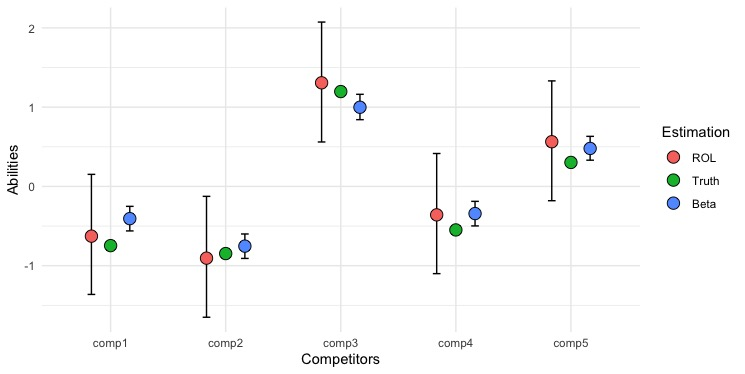
\includegraphics[scale=0.5]{images/Rplot01.jpeg}
\caption{True abilities and ROL and Beta estimated ones with 95\% credible intervals for five competitors}
\label{fig: ROL, Beta and true ability parameters for five competitors}
\end{figure}
\\
The analysis was conducted using package “CmdStanR” (\cite{gabry2021cmdstanr}) in R studio version 4.2.1 (\cite{posit2023rstudio}).


\addcontentsline{toc}{chapter}{References}
\printbibliography


\end{document}
